\subsubsection{Algoritmus RETE}
\label{rete}

Algoritmus RETE slouží k efektivnímu vyhodnocování splnění podmínek odvozovacích
pravidel (dále jen vyhodnocování). Je implementován dataflow sítí. Ta je
rozdělena do dvou částí, označovaných jako alpha a beta. Alpha část sítě
vyhodnocuje splnění jednotlivých podmínek pravidla fakty nově přidanými do či
odebranými z pracovní paměti. Beta část pak zajišťuje zachování konzistence
vazeb proměnných mezi podmínkami.

To, že je vyhodnocování sítí RETE tak efektivní, je zajištěno maximálním
sdílením častí sítě mezi pravidly. Mají-li dvě pravidla strukturálně stejný vzor
nějaké podmínky (liší se jen použité proměnné), sdílí tato pravidla část alpha
sítě, která tuto podmínku vyhodnocuje. Pokud mají dvě pravidla stejných několik
prvních podmínek, sdílí tato pravidla kromě části alpha sítě i část beta sítě,
která zajišťuje konzistenci vazeb proměnných mezi nimi. Čím více je v systému
definováno odvozovacích pravidel, tím pravděpodobnější jsou shody mezi jejich
podmínkami a tím více se efektivita algoritmu projeví.

Dataflow síť tvoří orientovaný acyklický
graf\footnote{\url{http://en.wikipedia.org/wiki/Directed\_acyclic\_graph}}. Uzly
sítě rozdělujeme na dva základní typy - paměťové a testovací. Paměťové uzly
ukládají průběžné výsledky vyhodnocování. Testovací uzly provádějí různé typy
testů (v závislosti na typu uzlu) nutných pro vyhodnocení podmínek pravidla.

Mezi uzly sítě dochází ke dvěma typům interakcí. Hlavním typem interakce je
aktivace. Ta probíhá ve směru hran grafu a uzel při ní provádí svou hlavní
funkci v~závislosti na typu. Testovací uzel se dále může dotazovat sousedního
paměťového uzlu na obsah jeho paměti a to \textbf{proti směru orientace hran}.
Abych odlišil sousední uzly ve směru hran (tedy ty, jež může uzel aktivovat) od
množiny všech sousedů, budu první skupinu nazývat \emph{potomky}.

Uzlu je při aktivaci vždy předána nějaká datová struktura. Tou je buď fakt, nebo
token, který reprezentuje posloupnost faktů. Zatímco paměťové uzly po aktivaci a
uložení datové struktury do své paměti vždy aktivují své potomky, testovací uzly
aktivují potomky jen v případě úspěšného testu.

Obrázek \ref{rete-alpha} zobrazuje úsek alpha části sítě RETE. Uzel
\verb|alpha-top-node| je vstupním bodem této sítě. Ten je aktivován při každé
změně pracovní paměti faktem, který byl přidán nebo odebrán. Potomky
\verb|alpha-top-nodu| jsou \verb|alpha-subtop-nody|, jeden pro jednoduché fakty
a jeden pro každou definovanou šablonu. \verb|Alpha-top-node| aktivuje příslušný
\verb|alpha-subtop-node| podle typu faktu. Ten pak aktivuje
\verb|alpha-test-node| pod ním.

Šrafované šipky v obrázku \ref{rete-alpha} symbolizují, že zde může následovat
posloupnost několika dalších \verb|alpha-test-nodů|. Každá cesta z
\verb|alpha-subtop-nodu| do \verb|alpha-memory-nodu| skrze posloupnost
\verb|alpha-test-nodů| vyhodnocuje jednu podmínku nějakého pravidla (případně
skupiny pravidel). Mějme například pravidla
\begin{minted}[samepage]{cl}
(defrule rule1
  (in :object box :location ?locaction)
  =>
  ...)
(defrule rule2
  (in :object box :location ?loc)
  =>
  ...).
\end{minted}
Tato pravidla mohou sdílet část alpha sítě pro vyhodnocení svých podmínek, neboť
ty se liší pouze názvy proměnných. Pro vyhodnocení těchto podmínek budeme
potřebovat jeden \verb|alpha-subtop-node| pro šablonu \verb|in|, jeden
\verb|alpha-test-node| pro testování, zda je hodnota slotu \verb|object| rovna
hodnotě \verb|box|, a jeden \verb|alpha-memory-node| pro uložení faktů, které
tuto podmínku splňují. Pro slot \verb|location| \verb|alpha-test-node|
nepotřebujeme, neboť alpha část sítě se hodnotami proměnných nezabývá.

\begin{figure}[h]
\centering
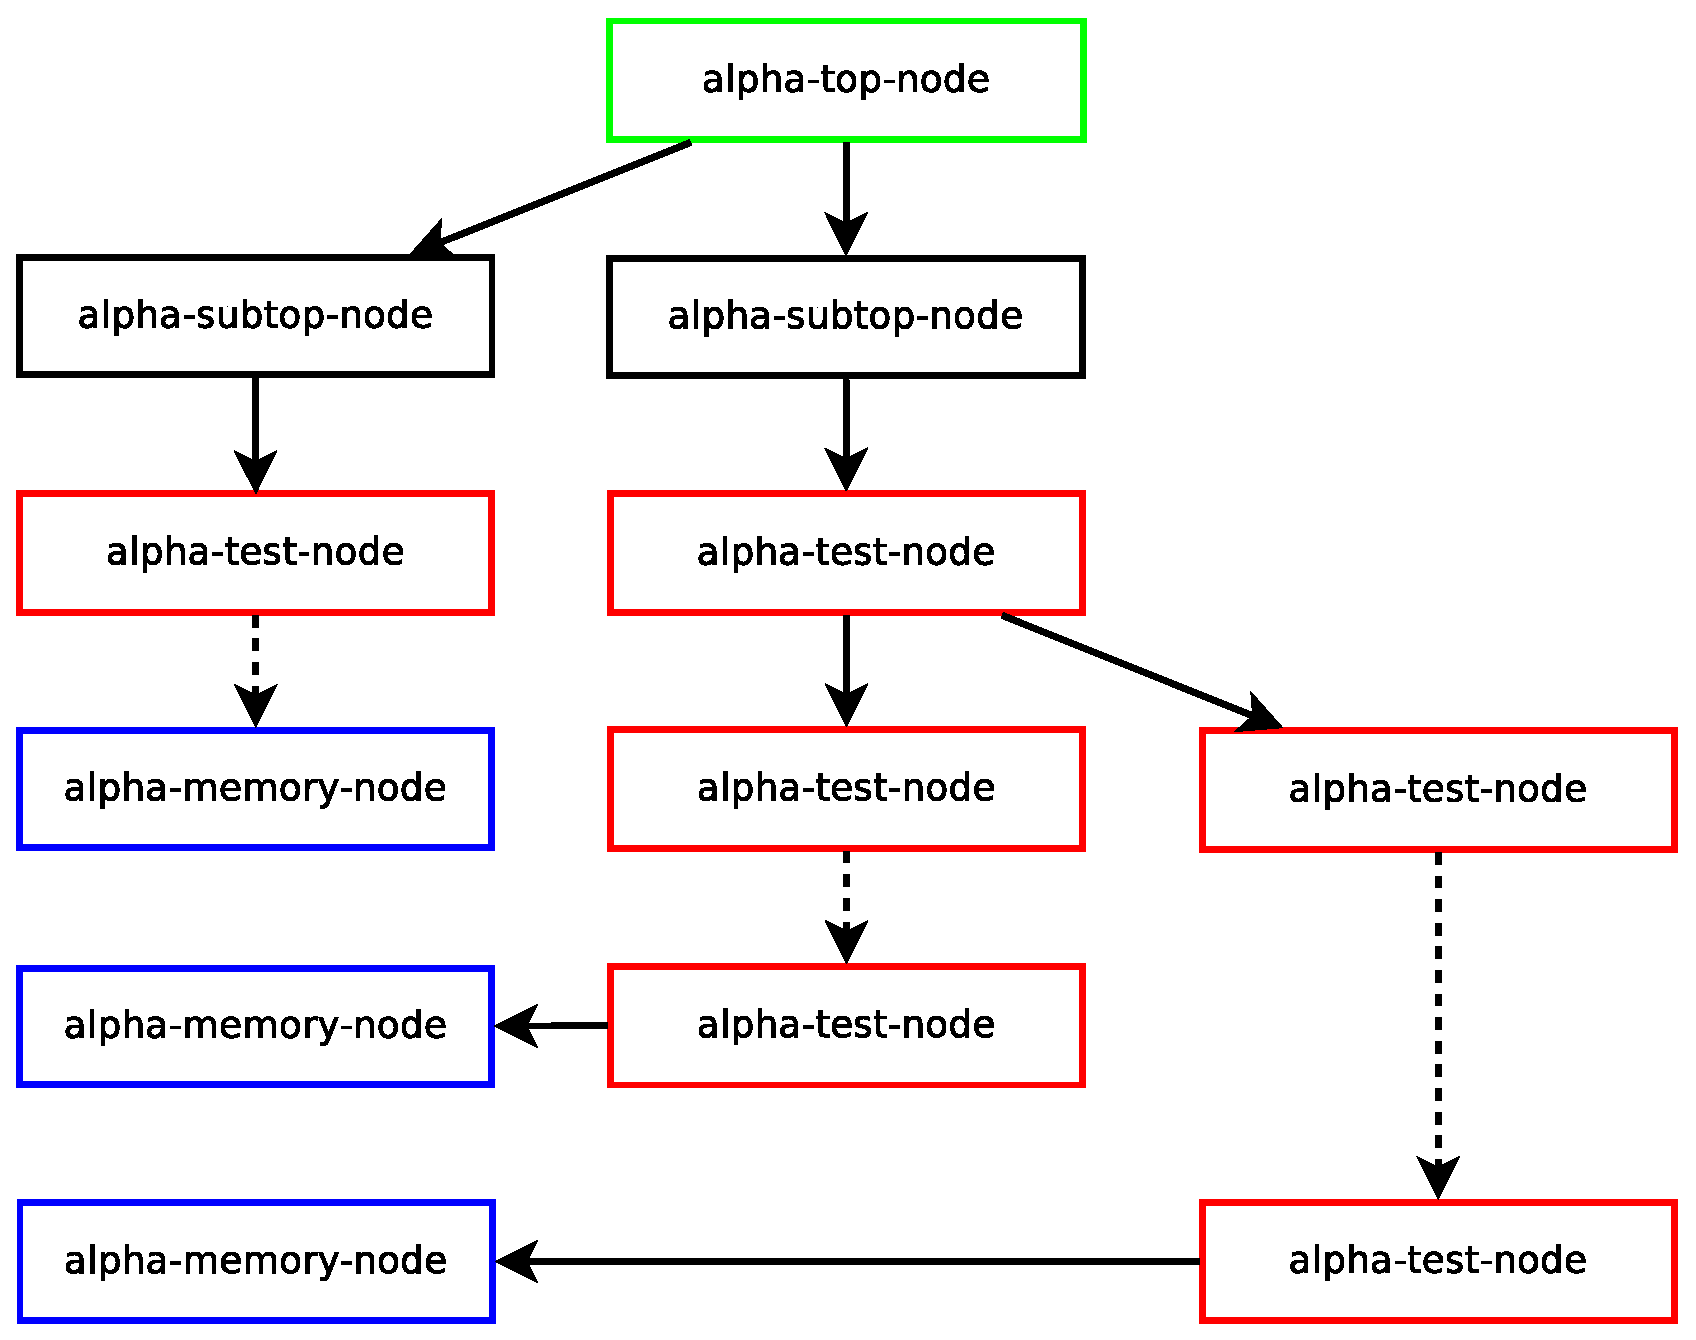
\includegraphics[height=10cm]{rete-alpha.eps}
\caption{Alpha část sítě RETE}
\label{rete-alpha}
\end{figure}

Obrázek \ref{rete-beta} zobrazuje úsek beta části sítě, spolu s
\verb|alpha-memory-nody|, kterými sem vstupují fakta splňující jednotlivé
podmínky pravidel. Každý \verb|beta-memory-node| udržuje množinu tokenů
reprezentujících posloupnosti faktů, z nichž každý splňuje podmínku nějakého
pravidla. \verb|Beta-join-nody| pak testují konzistenci vazeb proměnných mezi
těmito podmínkami. \verb|Beta-top-node| je speciální typ
\verb|beta-memory-nodu|, který udržuje v paměti pouze jeden prázdný token.
\verb|Production-node| je pak speciální typ \verb|beta-memory-nodu|, který
při aktivaci upozorní prostředí, že byly splněny všechny podmínky pravidla,
případně že po odstranění faktu už nejsou všechny splněny.

\begin{figure}[h]
\centering
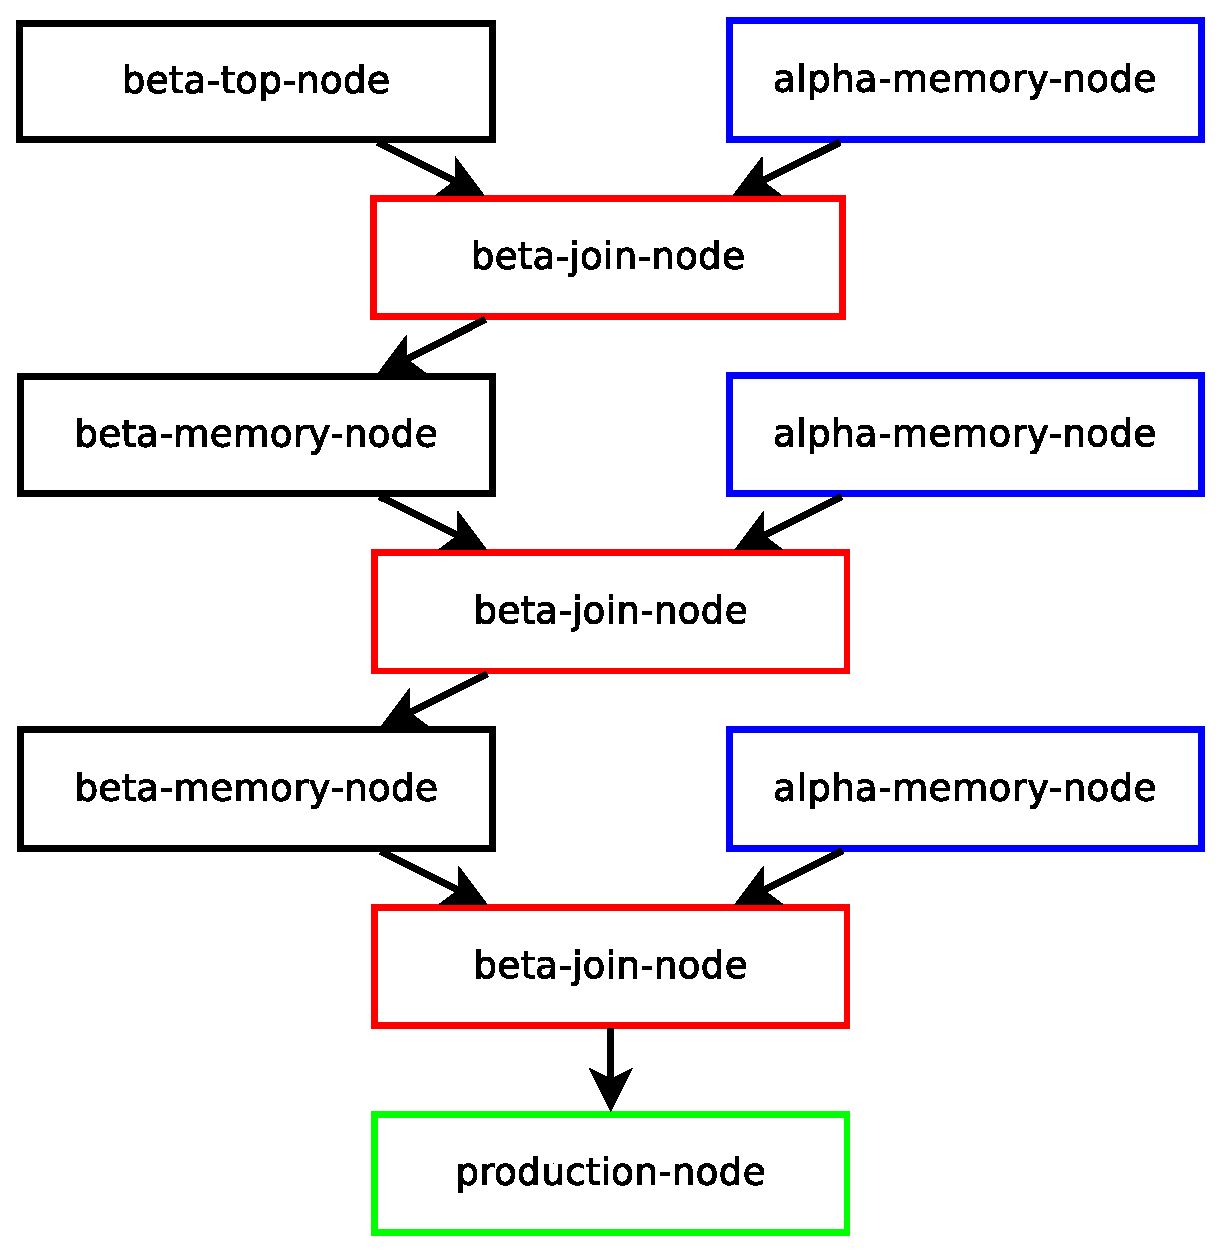
\includegraphics[height=10cm]{rete-beta.eps}
\caption{Beta část sítě RETE}
\label{rete-beta}
\end{figure}

Mějme například pravidlo
\begin{minted}[samepage]{cl}
(defrule rule
  (goal :object ?obj :from ?from :to ?to)
  (in :object ?obj :location ?from)
  (in :object robot :location ?to)
  =>
  ...).
\end{minted}
Alpha část sítě pro toto pravidlo bude obsahovat tři \verb|alpha-memory-nody|,
každý pro jednu jeho podmínku (kdyby však byla v poslední podmínce místo hodnoty
\verb|robot| proměnná, vystačili bychom si se dvěma \verb|alpha-memory-nody|).

Beta část sítě bude vypadat tak, jako na obrázku \ref{rete-beta} První (shora)
\verb|beta-test-node| ve skutečnosti nemá co testovat, neboť jde o první
podmínku pravidla. První \verb|beta-memory-node| bude udržovat tokeny délky 1
reprezentující \uv{posloupnost} faktů, které splňují první podmínku. Druhý
\verb|beta-join-node| bude testovat konzistenci vazeb mezi druhou a první
podmínkou pravidla. Druhý \verb|beta-memory-node| bude udržovat tokeny délky 2
reprezentující dvojice faktů, splňující první dvě podmínky pravidla. Třetí
\verb|beta-join-node| bude testovat konzistenci vazeb mezi třetí podmínkou
pravidla a předchozími dvěma. \verb|Production-node| pak bude udržovat tokeny
délky 3 reprezentující trojice faktů splňující všechny podmínky pravidla.

Přidávejme nyní postupně fakty do pracovní paměti. Přidáním
\verb|(in :object box :location A)| dojde (po průchodu alpha částí sítě)
k~aktivaci druhého \verb|alpha-memory-nodu|. Ten uloží fakt do své paměti a
aktivuje \uv{zprava} druhý \verb|beta-join-node|. Ten prohledá paměť
\verb|beta-memory-nodu| nad sebou, zda neobsahuje nějaký token s konzistentními
vazbami proměnných. Ta je ale prázdná, takže zde se aktivace zastaví.

Přidáním \verb|(goal :object box :from A :to B)| dojde k aktivaci prvního
\verb|alpha-memory-nodu|. Ten po uložení faktu aktivuje první
\verb|beta-join-node|. Ten nemá co testovat, takže aktivuje
\verb|beta-memory-node| pod sebou. Ten uloží jednoprvkový token s přidaným
faktem a aktivuje opět druhý \verb|beta-join-node|, tentokrát však \uv{zleva}.
\verb|Beta-join-node| tentokrát prohledá obsah paměti \verb|alpha-memory-nodu|
nad sebou, zda neobsahuje fakt konzistentní s tokenem. \verb|Beta-join-node| zde
testuje, zda jsou hodnoty slotů \verb|object| a \verb|location| faktu v alpha
paměti shodné s hodnotami \verb|object| a \verb|from| prvního faktu tokenu v
beta paměti.

Test zde skončí úspěšně, takže druhý \verb|beta-join-node| aktivuje
\verb|beta-memory-node| pod sebou a předá mu dvouprvkový token s oběma fakty.
Ten aktivuje \uv{zleva} třetí \verb|beta-join-node|. Ten následně prohledá paměť
\verb|alpha-memory-nodu| nad sebou. Ta je ale prázdná, takže zde aktivace
skončí.

Po přidání faktu \verb|(in :object robot :location B)| dojde k aktivaci třetího
\verb|alpha-memory-nodu|. Ten fakt uloží a aktivuje \uv{zprava} třetí
\verb|beta-join-node|. Ten prohledá paměť \verb|beta-memory-nodu| nad sebou, zda
neobsahuje konzistentní tokeny. Ta obsahuje dvouprvkový token s prvními dvěma
fakty. \verb|Beta-join-node| tedy srovná hodnotu slotu \verb|location| přidaného
faktu s hodnotou slotu \verb|to| prvního faktu tokenu. Protože tyto hodnoty se
shodují, aktivuje \verb|beta-join-node| \verb|production-node| pod sebou a předá
mu tříprvkový token s posloupností faktů, které splňují všechny podmínky
pravidla. Ten token uloží a upozorní prostředí, že pravidlo bylo splňeno
posloupností faktů v tokenu.

Jak jsme viděli, \verb|beta-join-node| může být aktivován buď zprava
\verb|alpha-memory-nodem| s novým faktem, který splňuje nějakou podmínku
pravidla, nebo zleva \verb|beta-memory-nodem| s tokenem, jehož fakty splňují
předchozí podmínky. V každém případě \verb|beta-join-node| prohledá obsah paměti
druhého paměťového uzlu nad ním, aby nalezl tokeny konzistentní s~novým faktem,
nebo fakty konzistentní s~novým tokenem.

Speciálním typem \verb|beta-join-nodu| je \verb|beta-negative-node|, který je
zprava aktivován \verb|alpha-memory-nodem| udržujícím fakty, které splňují
negovanou podmínku pravidla. Ten naopak testuje, že druhá paměť
\textbf{neobsahuje} konzistentní fakty/tokeny, a v takovém případě aktivuje
potomky.

Při odebrání faktu z pracovní paměti se síť chová velmi podobně. Paměťové uzly
ale v tomto případě odebírají fakty/tokeny ze svých pamětí.
Je-li při odebrání faktu aktivován \verb|production-node|, upozorní prostředí,
že pravidlo už není původní posloupností faktů splněno.

Odlišně se ovšem při odebrání faktu chovají \verb|beta-negative-nody|. Každý
\verb|beta-negative-node| je potomkem dvou paměťových uzlů - jednoho
\verb|beta-memory-nodu| a jednoho \verb|alpha-memory-nodu|. Pokud byl odebíraný
fakt/token v paměti jednoho z těchto paměťových uzlů jediným faktem/tokenem,
konzistentním s fakty/tokeny v druhém paměťovém uzlu, je nyní negovaná podmínka
pravidla splněna a \verb|beta-negative-node| aktivuje \verb|beta-memory-node|
pod sebou všemi tokeny z paměti \verb|beta-memory-nodu| nad sebou, jako by šlo o
nově přidané tokeny.

Kdybychom nyní přidali pravidlo, které má první dvě podmínky stejné jako
předchozí pravidlo, většina beta části sítě by zůstala stejná. Druhý
\verb|beta-memory-node| by ale získal jako potomka další \verb|beta-join-node|,
který by testoval konzistenci vazeb proměnných ve třetí, odlišné podmínce vůči
prvním dvěma. Pod ním by pak následovaly další uzly testující zbytek podmínek a
nový \verb|production-node|. Kdybychom přidali pravidlo, které má všechny
podmínky stejné, síť by se dokonce nezměnila vůbec. Původní
\verb|production-node| by si jen zapamatoval, že jeho aktivace nyní značí
splnění obou pravidel.

Každý typ uzlu sítě RETE je v programu reprezentován jedním typem objektu
stejného názvu. Každý z těchto objektů implementuje metodu \verb|activate|,
jejímž zavoláním je uzel aktivován. Většina kódu implementujícího modul
\verb|rete| je tvořena právě definicemi metod \verb|activate|. Další část kódu
pak implementuje dotváření sítě při přidání pravidla, které je netriviální.
Program zde prochází podmínky pravidla, přičemž zároveň postupuje v síti odshora
a zkoumá, zda je třeba vytvářet nové uzly, nebo lze použít existující, případně
je nově propojit.

Teorii potřebnou k implementaci algoritmu RETE jsem nastudoval z \cite{doorenbos}.
